\documentclass[
a4paper,     %% defines the paper size: a4paper (default), a5paper, letterpaper, ...
% landscape,   %% sets the orientation to landscape
% twoside,     %% changes to a two-page-layout (alternatively: oneside)
% twocolumn,   %% changes to a two-column-layout
% headsepline, %% add a horizontal line below the column title
% footsepline, %% add a horizontal line above the page footer
% titlepage,   %% only the titlepage (using titlepage-environment) appears on the first page (alternatively: notitlepage)
% parskip,     %% insert an empty line between two paragraphs (alternatively: halfparskip, ...)
% leqno,       %% equation numbers left (instead of right)
% fleqn,       %% equation left-justified (instead of centered)
% tablecaptionabove, %% captions of tables are above the tables (alternatively: tablecaptionbelow)
% draft,       %% produce only a draft version (mark lines that need manual edition and don't show graphics)
% 10pt         %% set default font size to 10 point
% 11pt         %% set default font size to 11 point
12pt         %% set default font size to 12 point
]{scrartcl}  %% article, see KOMA documentation (scrguide.dvi)


\usepackage{tikz}
\usetikzlibrary{arrows,automata}
\usepackage[latin1]{inputenc}
\usepackage[T1]{fontenc}
\usepackage{ae,aecompl}
\usepackage{amsmath,amssymb,amstext}
\usepackage{algorithm}
\usepackage{algpseudocode}
\usepackage{float}
\usepackage{psfrag}
\usepackage{listings}
\usepackage[automark]{scrpage2}
\usepackage{smartdiagram}
\usepackage{ifpdf}

\makeatletter
\def\BState{\State\hskip-\ALG@thistlm}
\makeatother


%%% Should be LAST usepackage-call!
%%% For docu on that, see reference on package ``hyperref''
\ifpdf%   (definitions for using pdflatex instead of latex)

  %%% graphicx: support for graphics

  \pdfcompresslevel=9

  %%% hyperref (hyperlinks in PDF): for more options or more detailed
  %%%          explanations, see the documentation of the hyperref-package
  \usepackage[%
    %%% general options
    pdftex=true,      %% sets up hyperref for use with the pdftex program
    %plainpages=false, %% set it to false, if pdflatex complains: ``destination with same identifier already exists''
    %
    %%% extension options
    backref,      %% adds a backlink text to the end of each item in the bibliography
    pagebackref=false, %% if true, creates backward references as a list of page numbers in the bibliography
    colorlinks=true,   %% turn on colored links (true is better for on-screen reading, false is better for printout versions)
    %
    %%% PDF-specific display options
    bookmarks=true,          %% if true, generate PDF bookmarks (requires two passes of pdflatex)
    bookmarksopen=false,     %% if true, show all PDF bookmarks expanded
    bookmarksnumbered=false, %% if true, add the section numbers to the bookmarks
    %pdfstartpage={1},        %% determines, on which page the PDF file is opened
    pdfpagemode=None         %% None, UseOutlines (=show bookmarks), UseThumbs (show thumbnails), FullScreen
  ]{hyperref}


  %%% provide all graphics (also) in this format, so you don't have
  %%% to add the file extensions to the \includegraphics-command
  %%% and/or you don't have to distinguish between generating
  %%% dvi/ps (through latex) and pdf (through pdflatex)
  \DeclareGraphicsExtensions{.pdf}

\else %else   (definitions for using latex instead of pdflatex)

  \usepackage[dvips]{graphicx}

  \DeclareGraphicsExtensions{.eps}

  \usepackage[%
    dvips,           %% sets up hyperref for use with the dvips driver
    colorlinks=false %% better for printout version; almost every hyperref-extension is eliminated by using dvips
  ]{hyperref}

\fi


%%% sets the PDF-Information options
%%% (see fields in Acrobat Reader: ``File -> Document properties -> Summary'')
%%% Note: this method is better than as options of the hyperref-package (options are expanded correctly)
\hypersetup{
  pdftitle={}, %%
  pdfauthor={}, %%
  pdfsubject={}, %%
  pdfcreator={Accomplished with LaTeX2e and pdfLaTeX with hyperref-package.}, %%
  pdfproducer={}, %%
  pdfkeywords={} %%
}


%%%%%%%%%%%%%%%%%%%%%%%%%%%%%%%%%%%%%%%%%%%%%%%%%%%%%%%%%%%%%%%%%%%%%%%%%%%%%%%%
%%%
%%% user defined commands
%%%

%%% \mygraphics{}{}{}
%% usage:   \mygraphics{width}{filename_without_extension}{caption}
%% example: \mygraphics{0.7\textwidth}{rolling_grandma}{This is my grandmother on inlinescates}
%% requires: package graphicx
%% provides: including centered pictures/graphics with a boldfaced caption below
%%
\newcommand{\mygraphics}[3]{
  \begin{center}
    \includegraphics[width=#1, keepaspectratio=true]{#2} \\
    \textbf{#3}
  \end{center}
}

%%%%%%%%%%%%%%%%%%%%%%%%%%%%%%%%%%%%%%%%%%%%%%%%%%%%%%%%%%%%%%%%%%%%%%%%%%%%%%%%
%%%
%%% define the titlepage
%%%

% \subject{}   %% subject which appears above titlehead
% \titlehead{} %% special heading for the titlepage

%%% title
\title{Seminarpaper}

%%% author(s)
\author{Mario Wagner, 0730223}

%%% date
\date{Graz, am \today{}}

% \publishers{}

% \thanks{} %% use it instead of footnotes (only on titlepage)

% \dedication{} %% generates a dedication-page after titlepage


%%% uncomment following lines, if you want to:
%%% reuse the maketitle-entries for hyperref-setup
%\newcommand\org@maketitle{}
%\let\org@maketitle\maketitle
%\def\maketitle{%
%  \hypersetup{
%    pdftitle={\@title},
%    pdfauthor={\@author}
%    pdfsubject={\@subject}
%  }%
%  \org@maketitle
%}


%%%%%%%%%%%%%%%%%%%%%%%%%%%%%%%%%%%%%%%%%%%%%%%%%%%%%%%%%%%%%%%%%%%%%%%%%%%%%%%%
%%%
%%% set heading and footer
%%%

%%% scrheadings default:
%%%      footer - middle: page number
%\pagestyle{scrheadings}

%%% user specific
%%% usage:
%%% \position[heading/footer for the titlepage]{heading/footer for the rest of the document}

%%% heading - left
% \ihead[]{}

%%% heading - center
% \chead[]{}

%%% heading - right
 \ohead[]{Seminar paper}

%%% footer - left
% \ifoot[]{}

%%% footer - center
% \cfoot[]{}

%%% footer - right
% \ofoot[]{}

\newcommand\me[1]{ [* {\textbf ME:} #1 *]}
\newcommand\mw[1]{ [* {\textbf MW:} #1 *]}


%%%%%%%%%%%%%%%%%%%%%%%%%%%%%%%%%%%%%%%%%%%%%%%%%%%%%%%%%%%%%%%%%%%%%%%%%%%%%%%%
%%%
%%% begin document
%%%

\begin{document}

\pagenumbering{roman} %% small roman page numbers

%%% include the title
% \thispagestyle{empty}  %% no header/footer (only) on this page
 \maketitle

%%% start a new page and display the table of contents
 %\newpage
 \tableofcontents

%%% start a new page and display the list of figures
%\newpage
\listoffigures

%%% start a new page and display the list of tables
% \newpage
 \listoftables

%%% display the main document on a new page
\newpage

\pagenumbering{arabic} %% normal page numbers (include it, if roman was used above)

%%%%%%%%%%%%%%%%%%%%%%%%%%%%%%%%%%%%%%%%%%%%%%%%%%%%%%%%%%%%%%%%%%%%%%%%%%%%%%%%
%%%
%%% begin main document
%%% structure: \section \subsection \subsubsection \paragraph \subparagraph
%%%
\section{Introduction}
Supervised learning is the task of inferring knowledge from a fully labeled training data. In contrast, unsupervised learning is the task of inferring knowledge from an unlabeled dataset. The common ground of supervised and unsupervised learning, is the task of inferring knowledge from a small amount of labeled data and a huge amount of unlabeled training data; i.e., \emph{semi-supervised learning}. In other words, semi-supervised learning is making use of that small amount of data (i.e., supervised learning) to do unsupervised learning considerably more accurate.
\par \emph{Active learning} is a special case of semi-supervised learning in which the labeled data is incrementally provided by a continuous interaction between the learner and an \emph{Oracle}. The oracle can be a user, a system, or a teacher that provides a certain level of insight to supervise the learner by letting it to actively query for labels of unknown data. When the oracle is a system, actively querying it only means the learner is iteratively providing the system with input alphabet and asking for the output alphabet.
\par This method is commonly used to learn models of reactive systems by actively providing them with external events (i.e., inputs) and observe how they react to them (i.e., outputs). Though, sometimes active learning can be as expensive as manual labeling since not all runs of all systems are inexpensive or repeatable; to exemplify, consider a scenario in which an input sequence triggers a safety critical behaviour of the system (e.g. self-termination).
\par \me{here goes a brief history about the L$^*$ algorithm of Angluin (2 or 3 paragraphs).}
\par Although L$^*$ is a quite useful automata learning approach, there are also issues with it; first of which is while using L$^*$ the learner either learns the correct system or nothing. Next issue with L$^*$ is actually stated earlier, that is, when it is impossible for some systems to perform some queries for various reasons (e.g. not being cost-effective, safety critical behaviour, expensive overheads, and etc.). Because of these reasons and many others that we may not know beforehand, passive learning (i.e., unsupervised learning) is used to learn the somewhat correct model of the system under learn. AALERGIA\cite{Mao.} is an interesting approach to learn stochastic automata from a data-set of traces of a system.
\par \me{here you have to reword parts of introduction of AALERGIA \cite{Mao.} that are relate to the incentives of devising such method; two or three paragraphs suffice.}

%%% Section PRELIMINARY
\newpage
\section{Preliminaries}
\subsection{Markov Models}
\subsubsection{Markov Decision Procedure}
\subsubsection{Deterministic Labeled Markov chain}
\subsubsection{Discrete-time Markov chain}
\subsection{Prism Model Checker}
\subsubsection{Probabilistic Linear Temporal Logic}
\me{That's on ME.}
\subsubsection{Dice Programs}
\me{(1) description, (2) graphical model top to bottom in tikz. (3) the prism code and its description. (4) what are we going to do with it? prism queries!}
\begin{figure}
  \centering
  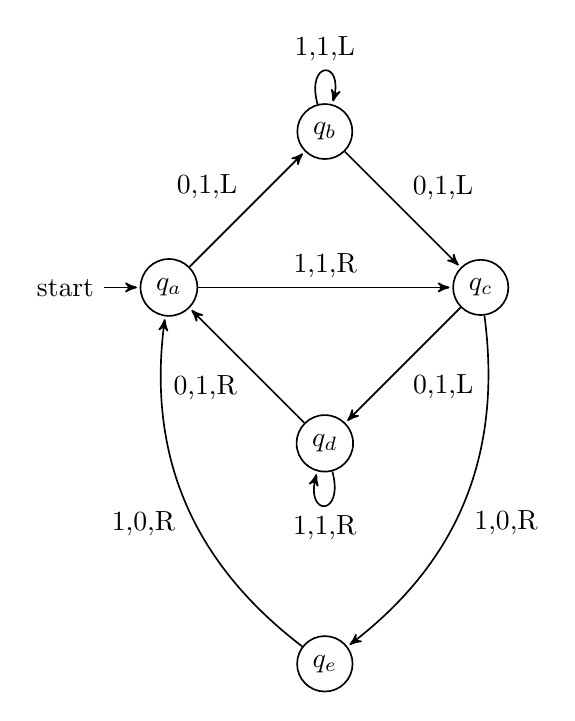
\begin{tikzpicture}[->,>=stealth',shorten >=1pt,auto,node distance=2.8cm,semithick]
  \tikzstyle{state}=[draw,circle,transform shape]
  \node[initial,state] (A)                    {$q_a$};
  \node[state]         (B) [above right of=A] {$q_b$};
  \node[state]         (D) [below right of=A] {$q_d$};
  \node[state]         (C) [below right of=B] {$q_c$};
  \node[state]         (E) [below of=D]       {$q_e$};
  \path [transform shape]
        (A) edge              node {0,1,L} (B)
            edge              node {1,1,R} (C)
        (B) edge [loop above] node {1,1,L} (B)
            edge              node {0,1,L} (C)
        (C) edge              node {0,1,L} (D)
            edge [bend left]  node {1,0,R} (E)
        (D) edge [loop below] node {1,1,R} (D)
            edge              node {0,1,R} (A)
        (E) edge [bend left]  node {1,0,R} (A);
\end{tikzpicture}
\caption{caption}\label{fig:something}
\end{figure}

\subsubsection{Herman's Self-Stabilisation Algorithm}
\me{(1) describe the problem; (2) how they handled the problem with prism model checker? (3) what are the findings? and be specific that we are going to use this case study from this point onward for the learning algorithm; otherwise we state that we are referring to the dice programs.}
\subsection{AALERGIA}
\me{(1) Who is responsible for ALERGIA; (2) Why they implemented this tool? (3) What are the issues with the tool?}
\me{(1) Who is responsible for AALERGIA; (2) How they addressed the issues with ALERGIA in this novel implementation? (3) Is there any room for improvement? (The answer is yes and you will refer to the PAutomataC contest + related work)}

In this paper, the algorithm AALERGIA\cite{Mao.} and the provided MATLAB implementation\footnote{http://mi.cs.aau.dk/code/aalergia} are used as a starting point for our work. In order to get a better idea of the way the implementation works, we will describe it in detail and a running example for better replicability is used throughout this section. The implementation of the algorithm consists of several parts, which are depicted in the figure~\ref{fig:diaAalergia}.

\begin{figure}[H]
\begin{center}
    \smartdiagramset{
        back arrow disabled=true,
        module minimum width=2cm,
    module minimum height=2cm,
    module x sep=3cm,
    text width=2cm,
    }
   \smartdiagram[flow diagram:horizontal]{Training Data, Prefix Tree Acceptor, Golden Section Search, AALERGIA, DLMC}
\end{center}
    \captionof{figure}{The Flow Diagram AALERGIA}
     \label{fig:diaAalergia}
\end{figure}

\subsubsection{Training Data}
The data used to learn the Deterministic Labeled Markov Chain (DLMC) is supplied in the form of a comma separated values file, which contains the training set and the alphabet to be used. The alphabet consists of a finite 1$\times$N-cell array, where each column contains one letter in the alphabet. The training set consist of a finite N$\times$1-cell array, where each row contains sequences of symbols generated from the model, separated by commas.
\paragraph{Dataset Generator} \me{we need to talk about how we are capable of generating dataset from a prism model.}
\par The running example we are going to use is a self-stabilizing ring network with 3 processes.
Table~\ref{table:trainingsSet} shows the beginning of the trainings set, which contains 50 Sequences in total.  In our case, each symbol in the training set represents the states in the ring at a given moment. For example, the symbol 001 shows that process 3 is in the state 1 and process 1 and 2 are in the state 0.

\begin{table}[ht!]
\centering
\begin{tabular}{|l|}
\hline
000,001,                                    \\ \hline
000,011,100,010,101,010,001,100,010,101,   \\ \hline
000,101,                                    \\ \hline
000,111,010,001,110,011,101,010,001,110,011, \\ \hline
000,111,011,101,110,001,                    \\ \hline
000,101,010,101,110,011,100,011,101,110,    \\ \hline
\end{tabular}
\caption{The Trainings set}
\label{table:trainingsSet}
\end{table}

Table~\ref{table:alphabet} shows the alphabet, which consists of 8 symbols from 000 to 111.

\begin{table}[ht!]
\centering
\begin{tabular}{|l|l|l|l|l|l|l|l|}
\hline
000 & 001 & 010 & 011 & 100 & 101 & 110 & 111 \\ \hline
\end{tabular}
\caption{The Alphabet}
\label{table:alphabet}
\end{table}

\subsubsection{Frequency Prefix Tree Acceptor}
After loading the trainings set and the alphabet into the workspace, the Frequency Prefix Tree Acceptor (FPTA) is created. A deterministic frequency finite automaton (DFFA) is a tuple $A = \langle \Sigma, Q, I\textsubscript{fr}, F\textsubscript{fr}, \delta\textsubscript{fr}, \delta \rangle$ where $ \Sigma $ = the finite alphabet, $Q$ = the finite set of states, $I\textsubscript{fr}$ = the initial state frequencies, $F\textsubscript{fr}$ = the final state frequencies, $\delta\textsubscript{fr}$ = the frequency transition function and $ \delta$ = the transition function. The frequency shows how often an event in the automaton occurs. \me{we need an example FPTA for dice programs here so the reader would depict an FPTA in his/her mind.}
\par Algorithm~\ref{alg:fpta} shows how the creation of the FPTA is implemented in the AALERGIA package. The code starts by sorting the trainings set and by removing double occurrences (line~\ref{fpta:sort}).
After that, a for-loop iterates through the sorted strings and splits them at each comma (line~\ref{fpta:BeginForPrefix} -~\ref{fpta:EndForPrefix}).
This creates all the prefixes from the trainings set and adds them to the cell array named \emph{prefix}, as shown in Table~\ref{table:prefix}.
\begin{table}[ht!]
\centering
\begin{tabular}{|l|}
\hline
000,000,010,001,100,011,101,110,001,110,001,110,011,101,010,001,100,011,100,010,001,   \\ \hline
000,000,010,001,100,011,101,110,001,110,001,110,011,101,010,001,100,011,100,010,   \\ \hline
000,000,010,001,100,011,101,110,001,110,001,110,011,101,010,001,100,011,100,   \\ \hline
000,000,010,001,100,011,101,110,001,110,001,110,011,101,010,001,100,011,   \\ \hline
000,000,010,001,100,011,101,110,001,110,001,110,011,101,010,001,100,   \\ \hline
000,000,010,001,100,011,101,110,001,110,001,110,011,101,010,001,   \\ \hline
000,000,010,001,100,011,101,110,001,110,001,110,011,101,010,   \\ \hline
000,000,010,001,100,011,101,110,001,110,001,110,011,101,   \\ \hline
000,000,010,001,100,011,101,110,001,110,001,110,011,   \\ \hline
000,000,010,001,100,011,101,110,001,110,001,110,   \\ \hline
000,000,010,001,100,011,101,110,001,110,001,   \\ \hline
\end{tabular}
\caption{The Prefixes}
\label{table:prefix}
\end{table}

\begin{algorithm}[H]
\caption{Create the FPTA}\label{alg:fpta}
\begin{algorithmic}[1]
\item \textbf{Input:} the $\sum$ and a set of strings S (training data)
\item \textbf{Output:} a DFFA A and a sorted set of strings U

\State $\textit{U} \gets \text{sort}(\textit{S})$ \label{fpta:sort}
\State $\textit{prefixes} \gets \textit{U}$
\State $\textit{F\textsubscript{fr}} \gets \text{string\_count}(\textit{U})$
\For{$\texttt{u} \in \texttt{U}$} \label{fpta:BeginForPrefix}
        \State $\textit{index} \gets \text{find positions of ``,'' in }\textit{u}$

        \While{$index > 0$}
          \State $\textit{substr} \gets \textit{substring(1:index)}$
         \If {$\textit{substr} \not\in \textit{prefix}$}
   	 \State $\textit{prefixes(end+1)} \gets \textit{substr}$
        \EndIf
           \State $\textit{index} \gets \textit{index-1}$
       \EndWhile
\EndFor \label{fpta:EndForPrefix}

\State $\textit{prefixes} \gets \text{width\_first\_sort}(\textit{prefixes})$ \label{fpta:widthSort}
\State $\textit{predecessor} \gets \text{find\_predecessor}(\textit{prefixes})$ \label{fpta:findPredecessor}

\For{$\texttt{p} \in \texttt{prefixes}$} \label{fpta:BeginForFreq}
\State $\textit{sym} \gets \textit{get\_symbol(p)}$
\State $\textit{pre} \gets \textit{predecessor(p)}$

\State $\textit{freq\_trans\_matrix\textsuperscript{1} (pre, sym)} \gets \textit{predecessor(p)}$
\State $\textit{frequency\_transition} \gets \textit{freq\_trans\_matrix\textsuperscript{2} (pre, sym)} $
\State $\textit{frequency\_transition} \gets \textit{frequency\_transition} + \textit{frequency(p)}$

 \While{$pre$}
          \State update\_freq\_trans\_matrix(\textit{p, pre})
          \State $\textit{pre} \gets \textit{predecessor(p)}$
   \EndWhile

\EndFor \label{fpta:EndForFreq}

\State $\textit{init\_states} \gets  \textit{freq\_trans\_matrix\textsuperscript{1}(1, all)}$
\State \Return \textit{A}  \label{fpta:return}
\end{algorithmic}
\end{algorithm}

In our example, the dimension of  \emph{prefix} is 494x1 and contains all unique prefixes of the trainings set for further evaluation.
The cell array \emph{prefix} is sorted by width-first-sort (line~\ref{fpta:widthSort}). The shortest strings are at the beginning of the array and the largest at the end of the array, as shown in Table~\ref{table:sortPrefix}.

\begin{table}[ht!]
\centering
\begin{tabular}{|l|}
\hline
000,         \\ \hline
000,000,     \\ \hline
000,001,     \\ \hline
000,010,     \\ \hline
000,011,     \\ \hline
000,100,     \\ \hline
000,101,     \\ \hline
000,110,     \\ \hline
000,111,     \\ \hline
000,000,010, \\ \hline
000,000,100, \\ \hline
000,000,111, \\ \hline
000,001,100, \\ \hline
000,001,110, \\ \hline
\end{tabular}
\caption{The Sorted Prefix Array}
\label{table:sortPrefix}
\end{table}

The function \emph{find\_predecessor} searches through the \emph{prefixes} array and saves all the predecessors in the corresponding array (line~\ref{fpta:widthSort}). In the end, a for-loop over all the prefixes is executed in order to find all transitions and their frequencies respectively. The values are saved into the \emph{freq\_trans\_matrix}  (line~\ref{fpta:BeginForFreq} -~\ref{fpta:EndForFreq}). This Matrix contains 2 elements: the first element is the transition matrix, which contains all the transition between the states. The second element is a matrix, which contains all the frequencies between the states.

The returned object DFFA (line~\ref{fpta:return}) has the following members:
\begin{itemize}
      \item a finite set of states
      \item the labels of the states
      \item the alphabet
      \item the initial state
      \item the initial state frequency
      \item the final state frequency
      \item the frequency transition matrix
      \item RED (later used for merging) \me{be more comprehensive about RED set}
      \item BLUE (later used for merging) \me{likewise}
   \end{itemize}

Table~\ref{table:transitionMatrix} shows how the first element of the frequency transition matrix (the transition matrix) is structured. The columns represent the 8 symbols, the rows the different states. For example,  row number 2, column 1 shows the number 3. This indicates that state 2 and symbol 1 lead to state 3. The second element of the frequency transition matrix has the same dimensions as the first element and follows the same logic, but instead of transitions it contains the frequencies.

\begin{table}[ht!]
\centering
\begin{tabular}{|l|l|l|l|l|l|l|l|}
\hline
2 & 0  & 0  & 0 & 0  & 0  & 0  & 0  \\ \hline
3 & 4  & 5  & 6 & 7  & 8  & 9  & 10 \\ \hline
0 & 0  & 11 & 0 & 12 & 0  & 0  & 13 \\ \hline
0 & 0  & 0  & 0 & 14 & 0  & 15 & 0  \\ \hline
0 & 16 & 0  & 0 & 0  & 17 & 0  & 0  \\ \hline
\end{tabular}
\caption{The Transition Matrix}
\label{table:transitionMatrix}
\end{table}

\subsubsection{Normalization}

The algorithm~\ref{alg:normalize} shows how a DFFA is converted into a deterministic probabilistic finite automaton (DPFA). The computation is pretty straightforward. As input, the algorithm takes a well defined DFFA, that means that the number of strings entering and leaving a given state is identical. The probabilistic transition matrix (line~\ref{normalize:ptm}) is identical to the frequency transition matrix, but its second element contains the probabilities of the transitions instead of the frequencies of the transitions.

The algorithm searches through the frequency transition matrix, sums up the frequencies of the transitions and adds them to the frequency of the state itself in order to get the total number of frequencies (line~\ref{normalize:sum}). Following that, the frequency of each transition and of the state is divided by the total number of total frequencies, which results in the corresponding probabilities for the transitions. (line~\ref{normalize:divide}).

\begin{algorithm}[H]
\caption{Create a DPFA from a DFFA}\label{alg:normalize}
\begin{algorithmic}[1]
\item \textbf{Input:} a well defined DFFA
\item \textbf{Output:} corresponding DPFA

\For{$q \in Q$}
        \State $\textit{freq\_state} \gets \textit{dffa.finalStateFrequency(q)}$
        \State $\textit{ptm\textsuperscript{1}} \gets \textit{dffa.frequencyTransitionMatrix\textsuperscript{1}}$ \label{normalize:ptm}
         \State $\textit{freq\_trans} \gets \textit{dffa.frequencyTransitionMatrix\textsuperscript{2}(q, all)}$
         \State $\textit{freq\_total} \gets \textit{freq\_trans + freq\_state}$  \label{normalize:sum}

         \If {$\textit{freq\_total} > 0$}
   	 \State $\textit{ptm\textsuperscript{2}(node, index)} \gets \frac{freq\_trans}{freq\_total}$ \label{normalize:divide}
   	  \State $\textit{fsp(q)} \gets \frac{freq\_state}{freq\_total}$
       \EndIf
\EndFor
\State \Return \textit{DPFA(dffa, fsp, ptm)}
\end{algorithmic}
\end{algorithm}

\subsubsection{Golden Section Search}

First, we need to search for a left and right border of $\varepsilon$ in order to get a region for our golden section search. This is done by the following algorithm~\ref{alg:findregion}. In order to save space, the algorithm only explains how to find the left border of the region. The right border is found the same way, with some minor modifications. The algorithm iteratively calculates BIC-scores for the values of $\varepsilon$. For each run of the while-loop, the $\varepsilon$ is multiplied by 0.5 until a left border is found. If the new $\varepsilon$ produces a Bayesian Information Criterion(BIC)-score larger than the previous $\varepsilon$ (line~\ref{findregion:scorelarger}), it essentially means that we found a right border, but the left border is further to the left and we need to search again. If the new score is the same as the old score  (line~\ref{findregion:scorethesame}), we search again. If the value of the score doesn't change for 5 consecutive tries, we break the loop and take the last value of $\varepsilon$ as our left border. Last but not least, if the new score is smaller than the old score (line~\ref{findregion:scoresmaller}), we found the left border and can continue searching for the right border (not shown in the pseudo code).
\paragraph{BIC Score} This is a measure that can be used to evaluate the learned model. It creates a score that is calculated on the likelihood minus a penalty term for the model complexity. A larger BIC score (x > y) means a better score and is preferred. Further details are given at \cite{Mao.}.
\me{we need the formula}

\begin{algorithm}[H]
\caption{Find $\varepsilon$-region}\label{alg:findregion}
\begin{algorithmic}[1]
\item \textbf{Input:} the DFFA
\item \textbf{Output:} the region for $\varepsilon$, scores, epsilon\_values

\State $\varepsilon \gets \textit{1}$
\State \textit{score} $\gets$ calculate\_BIC\_Score($\varepsilon$, \textit{dffa})
\State $new\_\varepsilon \gets \varepsilon * 0.5$

 \While{$new\_\varepsilon > 0$}

       \State \textit{new\_score} $\gets$ calculate\_BIC\_score(new\_$\varepsilon$, \textit{dffa})

         \If {\textit{new\_score > score}}  \label{findregion:scorelarger}
         \State $\textit{region\_right} \gets \varepsilon$
         \State $\varepsilon \gets new\_\varepsilon$
         \State $ new\_\varepsilon \gets new\_\varepsilon * 0.5$
         \State $\textit{score} \gets \textit{new\_score} $

         \ElsIf {\textit{new\_score = score}} \Comment{do this max. 5 times} \label{findregion:scorethesame}
   	 \State $\varepsilon \gets new\_\varepsilon$
         \State $ new\_\varepsilon \gets new\_\varepsilon * 0.5$
         \State $\textit{score} \gets \textit{new\_score} $

      \Else \label{findregion:scoresmaller}
      \State $\textit{region\_left} \gets new\_\varepsilon$
        \State break
       \EndIf

  \EndWhile

  \State ...
  \State ...

\State \Return \textit{region\_right, region\_left}
\end{algorithmic}
\end{algorithm}

Table~\ref{table:region} shows the values of the left and right border of $\varepsilon$. The algorithm ran only once for the left border ($\varepsilon$ startes with 1 and is halfed every run) and 5 times for the right border, since the scores always stayed the same. Table~\ref{table:bicscores} shows the BIC scores and table~\ref{table:epsilonvalues} shows the corresponding $\varepsilon$ values. For example, we calculated the BIC score for $\varepsilon = 0.5$ and the result was $-1.5769e+03$.

\begin{table}[ht!]
\centering
\begin{tabular}{|l|l|}
\hline
0.5 & 64 \\ \hline
\end{tabular}
\caption{The Search Region}
\label{table:region}
\end{table}

\begin{table}[ht!]
\centering
\begin{tabular}{|l|l|l|l|l|l|l|l|}
\hline
-840.6080 & -1.5769e+03 & -840.6080 & -840.6080 & -840.6080 & -840.6080 & -840.6080 & -840.6080 \\ \hline
\end{tabular}
\caption{The BIC scores}
\label{table:bicscores}
\end{table}

\begin{table}[ht!]
\centering
\begin{tabular}{|l|l|l|l|l|l|l|l|}
\hline
1 & 0.5 & 2 & 4 & 8 & 16 & 32 & 64 \\ \hline
\end{tabular}
\caption{The Epsilon values}
\label{table:epsilonvalues}
\end{table}

After having found the region, the golden section search can begin. Algorithm~\ref{alg:goldensection} shows how it is implemented. Basically, the algorithm uses the golden ratio on our 2 borders a1 and a2 and tries to find a maximum (the highest BIC score) between these 2 values. If it exists, the section that contains the maximum is selected as new region and the search is started again, until the recursion reaches depth 3 or the condition at line~\ref{golden:condition} is fulfilled. At line~\ref{golden:calcratio},~\ref{golden:calcratio2} we calculate the 2 values a1,a2 for our golden ratio, given the region r1,r2. After that, the corresponding BIC scores f1,f2 are calculated(line~\ref{golden:bicscore},~\ref{golden:bicscore2}). If the distance between the 2 values a1,a2 is small enough, we stop the recursion and the average score between the 2 values is taken as a good $\varepsilon$ (line~\ref{golden:average}). If f1 is smaller than f2, the maximum has to be between a1 and r2 and a new golden section search is started. If it is the other way around and f1 is larger than f2, the maximum is between r1 and a2 and we start the search with these values.
If it happens that the score of f1 and f2 is exactly the same, we need to make sure, that the recursion is not endless (line ~\ref{golden:limit}). We check if f1 is larger than the largest score we already calculated. Should this be the case, the maximum is between a1 and a2 (line~\ref{golden:maxscores}). Lastly, if we do not have any luck and we have not found a maximum so far, we simply start 2 new golden searches for the left (r1, a1) and the right (a2, r2) region respectively (line~\ref{golden:leftregion},~\ref{golden:rightregion}). In the end, the algorithm returns a suggestion for a good $\varepsilon$ as shown in Table~\ref{table:goodepsilon}, which we use as input parameter ($\alpha$) for our merging algorithm.

\begin{table}[ht!]
\centering
\begin{tabular}{|l|}
\hline
64 \\ \hline
\end{tabular}
\caption{The Epsilon}
\label{table:goodepsilon}
\end{table}

\begin{algorithm}[H]
\caption{Golden\_section\_search}\label{alg:goldensection}
\begin{algorithmic}[1]
\item \textbf{Input:} region, dffa, scores
\item \textbf{Output:} good\_eps, scores, epsilon

\State $\textit{good\_eps} \gets \textit{0}$
\State $\textit{r1} \gets \textit{region(1,1)}$
\State $\textit{r2} \gets \textit{region(1,2)}$

 \While{\textit{true}}

       \State $\textit{a1} \gets \textit{r1 + 0.382(r2-r1)}$ \label{golden:calcratio}
       \State $\textit{a2} \gets \textit{r2 + 0.618(r2-r1)}$ \label{golden:calcratio2}
       \State \textit{f1} $\gets$ calculate\_BIC\_score(\textit{a1,dffa}) \label{golden:bicscore}
       \State \textit{f2} $\gets$ calculate\_BIC\_score(\textit{a2, dffa}) \label{golden:bicscore2}

         \If {\textit{|a1-a2| < 0,00001}} \label{golden:condition}
       \State $\textit{good\_eps} \gets \textit{(a1 + a2) / 2}$   \label{golden:average}
        \State \Return
       \EndIf

        \If {\textit{f1 < f2}}
        \State $\textit{region} \gets \textit{region(a1, r2)}$
        \State \textit{good\_eps, scores, epsilon} $\gets$ Golden\_section\_search(\textit{region, dffa, scores})
       \State \Return

        \ElsIf {\textit{f1 > f2}}
        \State $\textit{region} \gets \textit{region(r1, a2)}$
        \State \textit{good\_eps, scores, epsilon} $\gets$ Golden\_section\_search(\textit{region, dffa, scores)}
        \State \Return

      \Else
        \If {\textit{recursion\_depth = 3}}  \label{golden:limit}
        \State \Return
        \EndIf

        \If {\textit{f1 > max(scores)}}  \label{golden:maxscores}
        \State $\textit{new\_region} \gets \textit{a1, a2)}$
        \State \textit{good\_eps, scores, epsilon} $\gets$ Golden\_section\_search(\textit{new\_region, dffa, scores)}
        \State \Return

        \Else
          \State $\textit{regionL} \gets \textit{region(r1, a1)}$
          \State $\textit{regionR} \gets \textit{region(a2, r2)}$
        \State \textit{good\_eps, scores, epsilon} $\gets$ Golden\_section\_search(\textit{regionL, dffa, scores)} \label{golden:leftregion}
         \State \textit{good\_eps, scores, epsilon} $\gets$ Golden\_section\_search(\textit{regionR, dffa, scores)} \label{golden:rightregion}
        \State \Return
        \EndIf
       \EndIf

  \EndWhile
\end{algorithmic}
\end{algorithm}

\subsubsection{Merging }

After having calculated a good $\alpha$ value, we can finally start the AALERGIA algorithm. RED is a set of states, that is already revised, whereas BLUE is the set of states that we need to look at. The RED set starts with the initial state (line~\ref{aalergia:redstart}) and BLUE gets all its successors (line~\ref{aalergia:bluestart}). After that, we loop through all the elements of BLUE and check if we can merge it with the AALERGIA\_compatible criterion (line~\ref{aalergia:criterion}). If the states are compatible, we can merge them and the tree becomes smaller, if not, we promote the state to the RED set (line~\ref{aalergia:promote}) and exclude it from the BLUE set (line~\ref{aalergia:excludeblue}). In the end, we get a merged DFFA with a good BIC score. Further details on the AALERGIA\_compatible criterion can be found at \cite{Mao.}

\begin{algorithm}[H]
\caption{AALERGIA}\label{alg:aalergia}
\begin{algorithmic}[1]
\item \textbf{Input:}  a DFFA, a DPFA, the alpha
\item \textbf{Output:} the merged DFFA

\State $\textit{RED} \gets \textit{dffa.initial\_state}$ \label{aalergia:redstart}
\State $\textit{BLUE} \gets \textit{freq\_trans\_matrix\textsuperscript{1}(dffa.initial\_state, all)}$ \label{aalergia:bluestart}
\State \textit{promote} $\gets$ \textit{1}

 \While{BLUE is not empty}

 \State $\textit{BLUE} \gets$ sort(\textit{BLUE})
 \State $\textit{q\_b} \gets \textit{BLUE(1)}$
 \State $\textit{BLUE}$.remove\textit{(q\_b)}
 \State $\textit{same\_label\_ind} \gets $find\_same\_labels(\textit{RED, q\_b)}

 \For{$ind \in same\_label\_ind$}
        \State $\textit{q\_r} \gets \textit{RED(ind)}$
        \State $\textit{threshold} \gets$ calculate\_compatible\_params(\textit{dffa, q\_r, q\_b, alpha})

        \If {AALERGIA\_compatible(\textit{dffa, dpfa, q\_r, q\_b, alpha, threshold})} \label{aalergia:criterion}
          \State \textit{dffa\_merged} $\gets$ AALERGIA\_merge(\textit{RED, BLUE, q\_r, q\_b})
          \State \textit{promote} $\gets$ \textit{0}
          \State break
        \EndIf
\EndFor

     \If  {promote}
          \State \textit{RED} $\gets$ \textit{q\_b} and \textit{RED} \label{aalergia:promote}
        \EndIf

    \State \textit{successors} $\gets$ \textit{dffa\_merged.freq\_trans\_matrix\textsuperscript{1}}(\textit{RED, all})
    \State \textit{BLUE} $\gets$ all \textit{successors} not in \textit{RED} \label{aalergia:excludeblue}
  \EndWhile
\end{algorithmic}
\end{algorithm}

\subsubsection{Perplexity}
%%% Section RELATED WORK
\newpage
\section{Related Work}
\me{The contest you were looking at. write three paragraphs each of which dedicated to one of the top three approaches; cite the publications (Worst to best).}
\me{The continue the discussion on SHIBATA and why it is winning every major contest in this field  PAutomataC 2012, CONTEST 2016.}

\section{Meat}
\me {a case study on wireless sensory networks.}



\newpage
\section{Evaluation}
\me {compare the findings about the case study with real-world scenario and the knowledge of an expert in the field of wireless sensory networks.}



\newpage
\section{Conclusions}
\me{the approach is good; but!}
%%%
%%% end main document
%%%
%%%%%%%%%%%%%%%%%%%%%%%%%%%%%%%%%%%%%%%%%%%%%%%%%%%%%%%%%%%%%%%%%%%%%%%%%%%%%%%%

\appendix  %% include it, if something (bibliography, index, ...) follows below

%%%%%%%%%%%%%%%%%%%%%%%%%%%%%%%%%%%%%%%%%%%%%%%%%%%%%%%%%%%%%%%%%%%%%%%%%%%%%%%%
%%%
%%% bibliography
%%%
%%% available styles: abbrv, acm, alpha, apalike, ieeetr, plain, siam, unsrt
%%%
 \bibliographystyle{ieeetr}

%%% name of the bibliography file
 \bibliography{sources}



\end{document}
%%% }}}
%%% END OF FILE
%%%%%%%%%%%%%%%%%%%%%%%%%%%%%%%%%%%%%%%%%%%%%%%%%%%%%%%%%%%%%%%%%%%%%%%%%%%%%%%%
%%% Notice!
%%% This file uses the outline-mode of emacs and the foldmethod of Vim.
%%% Press 'zi' to unfold the file in Vim.
%%% See ':help folding' for more information.
%%%%%%%%%%%%%%%%%%%%%%%%%%%%%%%%%%%%%%%%%%%%%%%%%%%%%%%%%%%%%%%%%%%%%%%%%%%%%%%%
%% Local Variables:
%% mode: outline-minor
%% OPToutline-regexp: "%% .*"
%% OPTeval: (hide-body)
%% emerge-set-combine-versions-template: "%a\n%b\n"
%% End:
%% vim:foldmethod=marker
% this is a test by Masoud 